\documentclass[11pt,a4paper]{article}

\usepackage[margin=21mm,headheight=15pt]{geometry}
\usepackage{amsmath,amssymb,mathtools}
\usepackage{booktabs,tabularx,array,longtable,multirow}
\usepackage{graphicx}
\usepackage{float}
\usepackage{xcolor}
\usepackage{fancyhdr}
\usepackage{tikz}
\usetikzlibrary{arrows.meta,positioning,fit,calc}
\usepackage[hidelinks]{hyperref}
\usepackage{xurl}
\usepackage{fontspec}

\setmainfont{TeX Gyre Pagella}
\setsansfont{TeX Gyre Heros}
\setmonofont{Latin Modern Mono}

\definecolor{navy}{HTML}{16324F}
\definecolor{blue}{HTML}{1B6CA8}
\definecolor{teal}{HTML}{168A83}
\definecolor{orange}{HTML}{D97706}
\definecolor{red}{HTML}{B83A3A}
\definecolor{green}{HTML}{287A4B}
\definecolor{lightblue}{HTML}{EDF6FC}
\definecolor{lightorange}{HTML}{FFF5E8}
\definecolor{lightgreen}{HTML}{EEF8F1}
\definecolor{lightgray}{HTML}{F4F6F8}

\setlength{\parindent}{0pt}
\setlength{\parskip}{5pt}
\setlength{\emergencystretch}{3em}
\setcounter{tocdepth}{2}

\pagestyle{fancy}
\fancyhf{}
\rhead{Latent graph-spectral representation redesign}
\lhead{SPECTRA-Siam}
\cfoot{\thepage}
\renewcommand{\headrulewidth}{0.4pt}

\newcommand{\R}{\mathbb{R}}
\newcommand{\concat}{\mathbin{\Vert}}
\newcommand{\sigmoid}{\operatorname{sigmoid}}
\newcommand{\LN}{\operatorname{LN}}
\newcommand{\Norm}{\operatorname{Normalize}_{2}}
\newcommand{\mean}{\operatorname{mean}}
\newcommand{\code}[1]{\texttt{#1}}
\newcommand{\yes}{\textcolor{green}{\textbf{Yes}}}
\newcommand{\no}{\textcolor{red}{\textbf{No}}}

\newenvironment{keybox}[1]{%
  \begin{center}\begin{minipage}{0.94\linewidth}
  \colorbox{lightblue}{\parbox{0.95\linewidth}{\textcolor{navy}{\textbf{#1}}\par\smallskip}}
  \vspace{-6pt}\begin{quote}
}{\end{quote}\end{minipage}\end{center}}

\title{\vspace{-12mm}\textbf{Evolution of the SPECTRA-Siam Representation}\\[3mm]
\Large Architecture and Results Report for SemanticCloneBench and AtCoder}
\author{Implementation-aligned technical report}
\date{August 15, 2026}

\begin{document}
\maketitle
\thispagestyle{empty}

\begin{abstract}
This report documents the evolution of SPECTRA-Siam from a legacy hybrid
readout to an attributed latent graph-spectral representation. In the legacy
model, canonical node categories and node-level lexical features affected
latent graph induction, but pooled latent-node states also reached the
classifier directly. One configuration additionally added a direct residual
from source tokens. Good scores from that system therefore could not be
attributed specifically to the learned graph spectrum. The first redesign
removed every direct feature path and retained only adjacency-spectrum
statistics. That design was methodologically clean but collapsed to nearly
single-class prediction. The second redesign preserves semantic information as
a signal on the learned latent graph and permits it to reach the classifier
only through graph-spectral filters. On the complete AtCoder test split of
116,736 pairs, the new model obtains F1=0.832, Accuracy=0.824,
Macro-F1=0.823, and ROC-AUC=0.893. The previous adjacency-only run predicted
every pair as positive and achieved Accuracy=0.500. The result is strong
evidence that the second redesign fixes the information bottleneck without
restoring the disputed direct lexical or node-state bypass.
\end{abstract}

\begin{center}
\fcolorbox{orange}{lightorange}{%
\begin{minipage}{0.92\linewidth}
\textbf{Claim boundary.}
The revised method is not an eigenvalue-only representation. Its accurate name
is an \emph{attributed latent graph-spectral representation} or
\emph{latent graph-signal spectral representation}. Node attributes remain in
the model, but they have no independent route to the classifier: their output
effect must be expressed through the learned Laplacian and the responses of
signals filtered on that Laplacian.
\end{minipage}}
\end{center}

\clearpage
{\small\tableofcontents}
\clearpage

\section{Executive conclusion}

The project contains three conceptually different systems that must not be
described as if they were the same method.

\begin{enumerate}
\item \textbf{Legacy hybrid readout.} The latent graph and a spectral descriptor
were learned, but the final program representation also received pooled latent
node states. The source-lexical configuration added another direct residual.
\item \textbf{First redesign: adjacency-only spectral readout.} All direct
feature paths were removed. The code embedding was computed only from spectral
density and heat-trace summaries of the learned latent adjacency. This version
collapsed.
\item \textbf{Second redesign: graph-signal spectral readout.} Node attributes
are retained as signals defined on the latent graph. The classifier sees only
eigenvalue summaries and permutation-invariant energies of signals after
Chebyshev graph-spectral filtering. No pooled node state or source-token
residual enters the output.
\end{enumerate}

\begin{keybox}{Main finding}
The problem was not the presence of lexical or canonical attributes. The
problem was their ability to bypass the graph-spectral operator. Removing both
the bypass and the attributed signal destroyed useful information. Reintroducing
the attributes only inside graph-spectral filtering restores useful separation
while preserving a defensible spectral latent-graph claim.
\end{keybox}

\section{Inputs and their exact roles}

The term \emph{lexical label} refers to an input attribute attached to a graph
node, not the target clone/non-clone label. Four input families are relevant.

\begin{table}[H]
\centering
\small
\begin{tabularx}{\linewidth}{p{0.18\linewidth}p{0.25\linewidth}Xp{0.16\linewidth}}
\toprule
Input family & Representation & Role in the revised method & Direct output path? \\
\midrule
Canonical type & One vocabulary identifier per graph node & Initial node state, relational message passing, latent graph induction, and latent graph signal & \no \\
Node lexical & Four bounded hashed identifiers per graph node & Gated addition to the canonical state, then graph induction and latent graph signal & \no \\
Source lexical & Hash sketch over the complete source text & Disabled in the revised method & \no \\
AST and DDG & Relation-specific adjacency tensors & Message passing, projected structural prior, and topology reconstruction target & Graph path only \\
\bottomrule
\end{tabularx}
\caption{Separation of input families and information routes.}
\end{table}

For input node $v$, the initial state is
\begin{align}
e_v^{\rm can}&=E_{\rm can}(\kappa_v),\\
e_v^{\rm lex}&=\frac{1}{4}\sum_{q=1}^{4}E_{\rm lex}(\ell_{vq}),\\
\gamma_{\rm lex}&=\sigmoid(g_{\rm lex}),\\
h_v^{(0)}&=M_v\,\LN\!\left(
e_v^{\rm can}+\gamma_{\rm lex}
\operatorname{Dropout}_{0.30}(e_v^{\rm lex})\right).
\end{align}
The lexical gate starts at approximately 0.20. The hashed lexical vocabulary
contains 4,096 buckets, and the hidden width is 256. Two relation-aware graph
layers operate on AST and DDG edges to produce
$H\in\R^{n\times256}$. At this point, attributes have influenced the graph
encoder, but no program-level feature has yet been sent to the pair classifier.

\section{Shared latent graph induction}

\subsection{Assignment to program-conditioned latent nodes}

Three slot-attention iterations map a variable-size input graph to 32 latent
nodes. The assignment matrix and latent states have shapes
$P\in\R^{n\times32}$ and $Z\in\R^{32\times256}$:
\begin{align}
P_{vj}&=\operatorname{softmax}_{j}
\left(\frac{Q(z_j)^\top K(h_v)}{\sqrt{256}}\right),\\
Z&=\operatorname{SlotUpdate}(H,P).
\end{align}
These are not persistent embeddings attached to dataset node identifiers.
They are program-conditioned latent states recomputed for each input using
shared model parameters.

\subsection{Structural prior and learned adjacency}

Observed AST and DDG topology is projected into the latent space:
\begin{equation}
B=P^\top A_{\rm obs}P,
\qquad
\widetilde B=\frac{B}{\max(B)+\epsilon}.
\end{equation}
Multi-head latent-node affinity is combined with this structural prior:
\begin{equation}
S=\operatorname{Sym}\left(
\frac{1}{4}\sum_{h=1}^{4}
\frac{Q_h(Z)K_h(Z)^\top}{\sqrt{64}}
\right)+\eta\widetilde B.
\end{equation}
The revised implementation retains a differentiable weighted adjacency:
\begin{equation}
A_\Theta=\operatorname{Sym}\left[
\sigmoid\left(S/\tau(c)\right)\odot
(\mathbf 1\mathbf 1^\top-I)\right].
\end{equation}
The temperature $\tau(c)$ is adapted from input complexity. A fixed
\code{top-k=3} graph is not used in the second redesign because forcing nearly
identical edge counts across examples suppresses the graph-to-graph spectral
variation required by the readout. Two latent graph refinement layers then
produce final latent states $Z'$.

\section{Legacy method: hybrid readout and attribution ambiguity}

The legacy system computed a 152-dimensional spectral descriptor:
\begin{equation}
s_\Theta=d(\lambda)\concat h(\lambda)\concat
\operatorname{vec}(E_{\rm Cheb})
\in\R^{32+24+96}.
\end{equation}
It projected that descriptor to a spectral embedding, but then concatenated a
direct average of latent-node states:
\begin{align}
z_{\rm spec}&=\operatorname{GELU}
\left(W_{\rm spec}\LN(s_\Theta)+b_{\rm spec}\right),\\
\bar z&=\frac{1}{32}\sum_{j=1}^{32}z'_j,\\
\phi_{\rm old}&=\Norm\left(
\operatorname{MLP}(\bar z\concat z_{\rm spec})\right).
\end{align}
The source-lexical configuration added a further direct residual:
\begin{equation}
\phi_{\rm old+src}=\Norm\left(
\phi_{\rm old}+\gamma_{\rm src}z_{\rm src}\right).
\end{equation}

\begin{figure}[H]
\centering
\resizebox{\linewidth}{!}{%
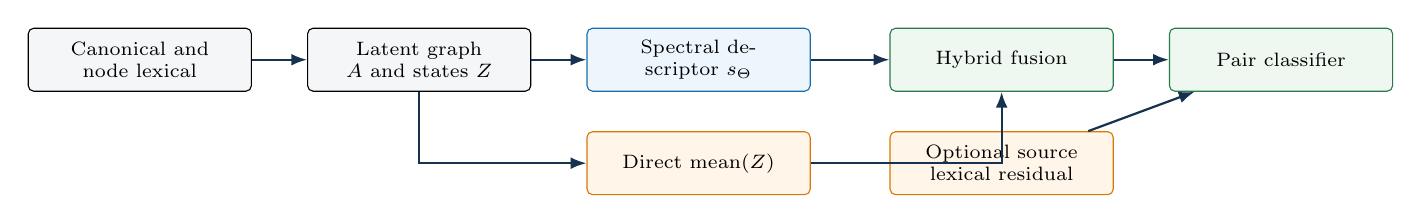
\begin{tikzpicture}[
  node distance=5mm and 7mm,
  box/.style={draw,rounded corners=2pt,align=center,minimum height=8mm,
    text width=26mm,font=\scriptsize,fill=lightgray},
  spec/.style={box,fill=lightblue,draw=blue},
  bypass/.style={box,fill=lightorange,draw=orange},
  outputbox/.style={box,fill=lightgreen,draw=green},
  arr/.style={-{Latex[length=2mm]},thick,draw=navy}
]
\node[box] (input) {Canonical and node lexical};
\node[box,right=of input] (latent) {Latent graph $A$ and states $Z$};
\node[spec,right=of latent] (spectral) {Spectral descriptor $s_\Theta$};
\node[bypass,below=of spectral] (pool) {Direct $\operatorname{mean}(Z)$};
\node[outputbox,right=10mm of spectral] (fusion) {Hybrid fusion};
\node[bypass,below=of fusion] (source) {Optional source lexical residual};
\node[outputbox,right=of fusion] (classifier) {Pair classifier};
\draw[arr] (input)--(latent);
\draw[arr] (latent)--(spectral);
\draw[arr] (latent)|-(pool);
\draw[arr] (spectral)--(fusion);
\draw[arr] (pool)-|(fusion);
\draw[arr] (fusion)--(classifier);
\draw[arr] (source)--(classifier);
\end{tikzpicture}}
\caption{Legacy hybrid architecture. Orange branches reach the output without
mandatory graph-spectral filtering.}
\end{figure}

If the classifier obtains a useful decision boundary from $\bar z$ or
$z_{\rm src}$, strong performance demonstrates a successful hybrid
graph-feature model. It does not demonstrate that the learned latent graph
spectrum is the principal source of discrimination. This was the central
methodological objection to the legacy paper-facing interpretation.

\section{First redesign: adjacency-only spectral readout}

The first redesign removed the direct node-state and source-token branches.
The normalized latent Laplacian was
\begin{equation}
L=I-D^{-1/2}A_\Theta D^{-1/2}.
\end{equation}
Only two families of eigenvalue-derived statistics were retained:
\begin{align}
d_r(\lambda)&=\frac{1}{32}\sum_{i=1}^{32}
\exp\left[-\frac{(\lambda_i-c_r)^2}{2(0.08)^2}\right],
\qquad r=1,\ldots,32,\\
h_t(\lambda)&=\frac{1}{32}\sum_{i=1}^{32}\exp(-t\lambda_i),
\qquad t\in\operatorname{logspace}(-2,2,24).
\end{align}
Thus the complete program descriptor had only $32+24=56$ dimensions and was a
function of $A_\Theta$ alone. Canonical and lexical information could affect
the prediction only if graph induction successfully encoded it into the
adjacency spectrum.

\begin{table}[H]
\centering
\small
\begin{tabular}{lrrrrrrrr}
\toprule
Dataset & P & R & F1 & Acc & Macro-F1 & BA & AUC & Positive rate \\
\midrule
SemanticCloneBench & 0.505 & 0.974 & 0.665 & 0.510 & 0.376 & 0.510 & 0.601 & 0.964 \\
AtCoder & 0.500 & 1.000 & 0.667 & 0.500 & 0.333 & 0.500 & 0.498 & 1.000 \\
\bottomrule
\end{tabular}
\caption{Two independent signs of failure for the adjacency-only readout.}
\end{table}

On SemanticCloneBench, the run correctly identified only 25 of 539 negative
pairs: $TN=25$, $FP=514$, $TP=525$, and $FN=14$. Its probabilities were almost
constant, with mean 0.498775 and standard deviation 0.000663. On AtCoder, the
failure was complete: $TP=58{,}368$, $FP=58{,}368$, $TN=0$, and $FN=0$.
Positive-class F1 remained 0.667 only because an all-positive classifier on a
balanced dataset has recall 1.0. Macro-F1 and Balanced Accuracy exposed the
collapse.

Four mechanisms are consistent with this failure:
\begin{enumerate}
\item The adjacency spectrum is a many-to-one summary. Structurally different
graphs can have very similar spectra or can be cospectral.
\item Attribute information passed through the severe bottleneck
$X\rightarrow A_\Theta\rightarrow\lambda(L)$ before reaching the classifier.
\item Fixed \code{top-k=3} sparsification made edge counts and spectra too
similar across examples.
\item Checkpoint selection led with positive-class F1, which can prefer a
nearly all-positive solution on a balanced dataset.
\end{enumerate}

\section{Second redesign: attributed graph-signal spectral readout}

\subsection{Latent graph signal}

The second redesign does not concatenate semantic information beside the
spectrum. Instead, final latent states are projected to eight signal channels
and normalized across graph nodes:
\begin{equation}
X=\frac{Z'W_s}{
\sqrt{\mean_v(Z'W_s)^2+\epsilon}}
\in\R^{32\times8}.
\end{equation}
RMS normalization prevents the raw scale of $Z'W_s$ from functioning as a
non-spectral shortcut. Information must be expressed through its distribution
over graph frequencies.

\subsection{Chebyshev graph-spectral filter bank}

Twelve Gaussian spectral bands are approximated with degree-12 Chebyshev
polynomials. With $\widetilde L=L-I$, the recurrence is
\begin{align}
T_0(\widetilde L)X&=X,\\
T_1(\widetilde L)X&=\widetilde L X,\\
T_k(\widetilde L)X&=2\widetilde L T_{k-1}(\widetilde L)X
-T_{k-2}(\widetilde L)X.
\end{align}
For band $b$ and channel $q$,
\begin{align}
Y_{bq}&=g_b(L)X_q\simeq
\sum_{k=0}^{12}c_{bk}T_k(L-I)X_q,\\
e_{bq}&=\log\left(1+
\frac{1}{32}\sum_{v=1}^{32}Y_{bq}(v)^2\right).
\end{align}
Squaring and averaging over nodes makes the energy invariant to permutations
of latent-node order. The descriptor is
\begin{equation}
s=\left[
\underbrace{d(\lambda)}_{32};
\underbrace{h(\lambda)}_{24};
\underbrace{\operatorname{vec}(e)}_{12\times8=96}
\right]\in\R^{152}.
\end{equation}
It is projected to a normalized 256-dimensional program embedding. The
graph-signal bands are fixed rather than weighted by input-conditioned node
attention, preventing a hidden state-dependent gate from becoming another
bypass.

\subsection{Pair comparison}

For two program embeddings $u,v\in\R^{256}$, the pair classifier receives
\begin{equation}
r(u,v)=u\concat v\concat|u-v|\concat(u\odot v)
\concat\operatorname{cos}(u,v)\in\R^{1025}.
\end{equation}
The classifier never sees raw canonical identifiers, lexical hashes, pooled
node states, or source-token features.

\begin{figure}[H]
\centering
\resizebox{\linewidth}{!}{%
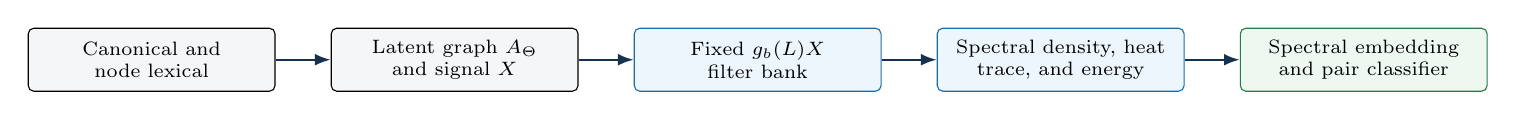
\begin{tikzpicture}[
  node distance=5mm and 7mm,
  box/.style={draw,rounded corners=2pt,align=center,minimum height=8mm,
    text width=29mm,font=\scriptsize,fill=lightgray},
  spec/.style={box,fill=lightblue,draw=blue},
  outputbox/.style={box,fill=lightgreen,draw=green},
  arr/.style={-{Latex[length=2mm]},thick,draw=navy}
]
\node[box] (input) {Canonical and node lexical};
\node[box,right=of input] (latent) {Latent graph $A_\Theta$ and signal $X$};
\node[spec,right=of latent] (filter) {Fixed $g_b(L)X$ filter bank};
\node[spec,right=of filter] (energy) {Spectral density, heat trace, and energy};
\node[outputbox,right=of energy] (classifier) {Spectral embedding and pair classifier};
\draw[arr] (input)--(latent);
\draw[arr] (latent)--(filter);
\draw[arr] (filter)--(energy);
\draw[arr] (energy)--(classifier);
\end{tikzpicture}}
\caption{Second redesign. Every attribute-dependent output path crosses a
polynomial function of the learned latent Laplacian.}
\end{figure}

\section{Exact information-route comparison}

\begin{table}[H]
\centering
\small
\begin{tabularx}{\linewidth}{p{0.25\linewidth}XXX}
\toprule
Property & Legacy hybrid & Adjacency-only & Graph-signal spectral \\
\midrule
Node lexical affects $A_\Theta$ & \yes & \yes & \yes \\
Attributes preserved in output & Direct state and spectral paths & Only if encoded in $A_\Theta$ & Only through $g_b(L)X$ \\
Direct $\mean(Z')$ & \yes & \no & \no \\
Source lexical residual & Optional and direct & \no & \no \\
Input-conditioned band gate & Optional & Not applicable & \no; fixed bands \\
Final encoder input & $[z_{\rm spec};\mean(Z')]$ & Spectrum of $A_\Theta$ & Spectrum and filtered-signal energies \\
Correct scientific label & Hybrid graph-feature model & Latent topology spectrum & Attributed latent graph-spectral model \\
Attribution clarity & Ambiguous & Clear but insufficient & Clear within the attributed spectral framework \\
\bottomrule
\end{tabularx}
\caption{Causal comparison of the three readout families.}
\end{table}

\begin{keybox}{Direct answer about lexical information}
In the revised model, lexical and canonical features still influence the
learned graph. They also remain available as a signal defined on that graph.
However, they are not fused into the final representation as an independent
vector. Their observable contribution must appear in the response
$g_b(L)X$ or in the spectrum of $L$. Therefore, the revised model preserves
semantic information without restoring the legacy shortcut.
\end{keybox}

\section{Training and evaluation protocol}

The collapse showed that architecture and model selection both required
changes.

\begin{table}[H]
\centering
\small
\begin{tabularx}{\linewidth}{p{0.27\linewidth}p{0.29\linewidth}X}
\toprule
Component & First redesign & Second redesign \\
\midrule
Latent adjacency & Fixed top-k, nearly fixed edge count & Soft, symmetric, weighted adjacency \\
Band weighting & State-dependent attention available & Fixed equal bands \\
Checkpoint selection & Positive F1 first & ROC-AUC, then Macro-F1, then Balanced Accuracy \\
Threshold selection & Positive F1 first & Macro-F1, then Balanced Accuracy, then F1 \\
Collapse warning & Too narrow & Probability std below 0.005 or class rate outside 5--95 percent \\
SemanticCloneBench schedule & Four diagnostic epochs & Up to 30 epochs, minimum 10, patience 6 \\
AtCoder schedule & Four epochs & Four epochs in the reported run \\
\bottomrule
\end{tabularx}
\caption{Changes that improve spectral variation and prevent single-class
checkpoint selection.}
\end{table}

The multi-objective training loss is
\begin{align}
\mathcal L={}&\mathcal L_{\rm cls}
+0.30\mathcal L_{\rm spectral\ pair}
+0.20\mathcal L_{\rm hard\ neg}
+0.05\mathcal L_{\rm node\ rec}\\
&+0.05\mathcal L_{\rm topology\ rec}
+0.05\mathcal L_{\rm variance}
+0.01\mathcal L_{\rm graph}.
\end{align}
Topology reconstruction pushes $PA_\Theta P^\top$ toward observed AST+DDG
structure. Node reconstruction regularizes the latent assignment. The
variance term discourages constant spectral embeddings, while the graph term
regularizes density and connectivity.

\section{Evidence sources and comparison limits}

This report separates four local evidence sources:
\begin{enumerate}
\item Historical paper results in \code{paper/results.tex} for Topology only,
Graph + labels, and Graph + labels + source lexical.
\item \code{results.zip}, containing raw predictions, history, metrics, and
metadata for the adjacency-only SemanticCloneBench run.
\item The recorded summary of the previous adjacency-only AtCoder run. Its raw
prediction archive is not present in the current workspace.
\item \code{atcoder result.zip}, containing the complete graph-signal spectral
AtCoder run. Every reported test metric for this run was independently
recomputed from 116,736 raw predictions and matches the notebook JSON and CSV.
\end{enumerate}

Historical rows are useful performance references, but they were not all
generated with identical checkpoint criteria and architecture details. The
strongest current evidence is the removal of collapse in the new AtCoder run.
Several design and training changes were introduced together, so the exact
contribution of each component still requires controlled ablation.

\section{New AtCoder result}

The run used seed 42, one Tesla T4 GPU, four epochs, and every graph-evaluable
pair: 544,054 training pairs, 116,704 validation pairs, and 116,736 test
pairs. The test split is exactly balanced with 58,368 clone and 58,368
non-clone pairs. The model has 3,013,429 trainable parameters.

\begin{table}[H]
\centering
\small
\begin{tabular}{lrrrrrrrr}
\toprule
Split & P & R & F1 & Acc & Macro-F1 & BA & AUC & Threshold \\
\midrule
Validation & 0.8076 & 0.8400 & 0.8235 & 0.8200 & 0.8199 & 0.8200 & 0.9028 & 0.3740 \\
Test & 0.7950 & 0.8723 & 0.8319 & 0.8237 & 0.8233 & 0.8237 & 0.8932 & 0.3740 \\
\bottomrule
\end{tabular}
\caption{Graph-signal spectral results. The threshold was selected only on
validation and then applied unchanged to test.}
\end{table}

The test confusion matrix is $TP=50{,}917$, $FP=13{,}133$,
$TN=45{,}235$, and $FN=7{,}451$. The predicted-positive rate is 0.5487, so the
model has not collapsed to either class. Independent metrics recomputed from
the raw prediction archive are MCC=0.6504, PR-AUC=0.8646, Brier score=0.1342,
and log loss=0.4493.

Probability distributions also show real class separation. The mean clone
probability is 0.2019 for non-clones and 0.7633 for clones; the medians are
0.0186 and 0.8906, respectively. Overall probability standard deviation is
0.4057, compared with 0.000663 in the collapsed SemanticCloneBench run. This
improvement is not merely a threshold artifact because ROC-AUC is 0.893.

\begin{figure}[H]
\centering
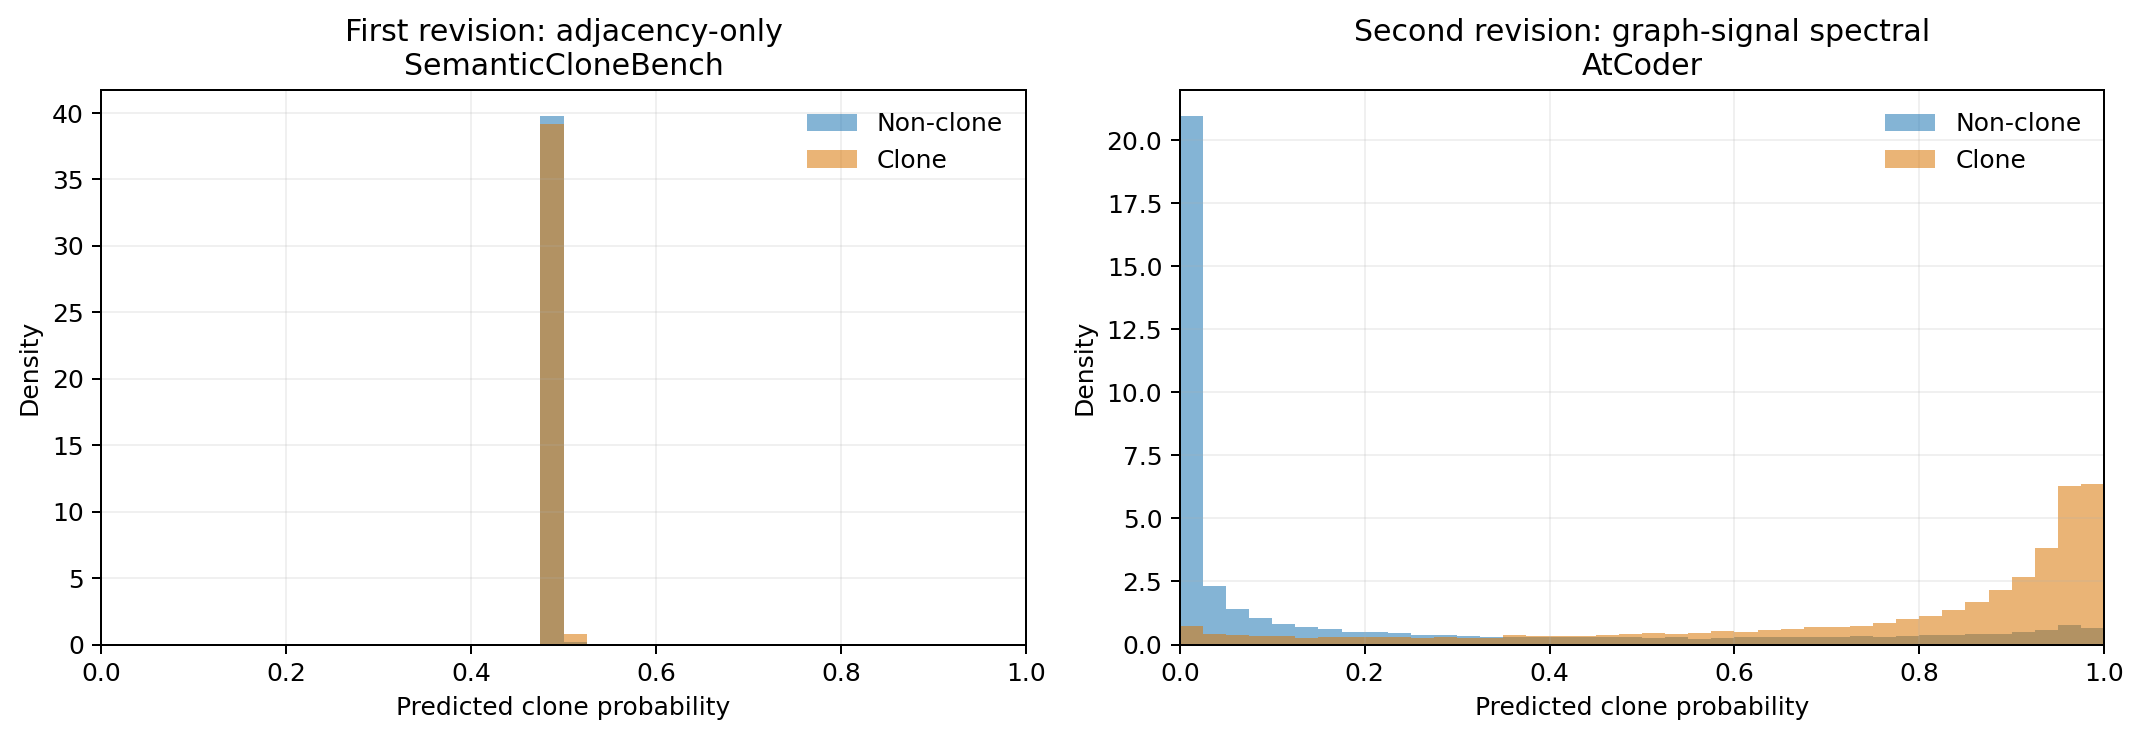
\includegraphics[width=\linewidth]{assets/method_evolution/probability_separation_comparison.png}
\caption{Left: near-constant probabilities from the first redesign on
SemanticCloneBench. Right: broad class separation from the second redesign on
AtCoder. The panels use different datasets and illustrate collapse rather than
constituting a direct cross-dataset statistical test.}
\end{figure}

\subsection{Training trajectory}

\begin{table}[H]
\centering
\small
\begin{tabular}{rrrrr}
\toprule
Epoch & Train loss & Valid F1 & Valid Macro-F1 & Valid AUC \\
\midrule
1 & 0.7093 & 0.7518 & 0.7415 & 0.8183 \\
2 & 0.4771 & 0.7949 & 0.7873 & 0.8634 \\
3 & 0.3898 & 0.8108 & 0.8081 & 0.8874 \\
4 & 0.3346 & 0.8235 & 0.8199 & 0.9028 \\
\bottomrule
\end{tabular}
\caption{Complete training history for the new AtCoder run.}
\end{table}

\begin{figure}[H]
\centering
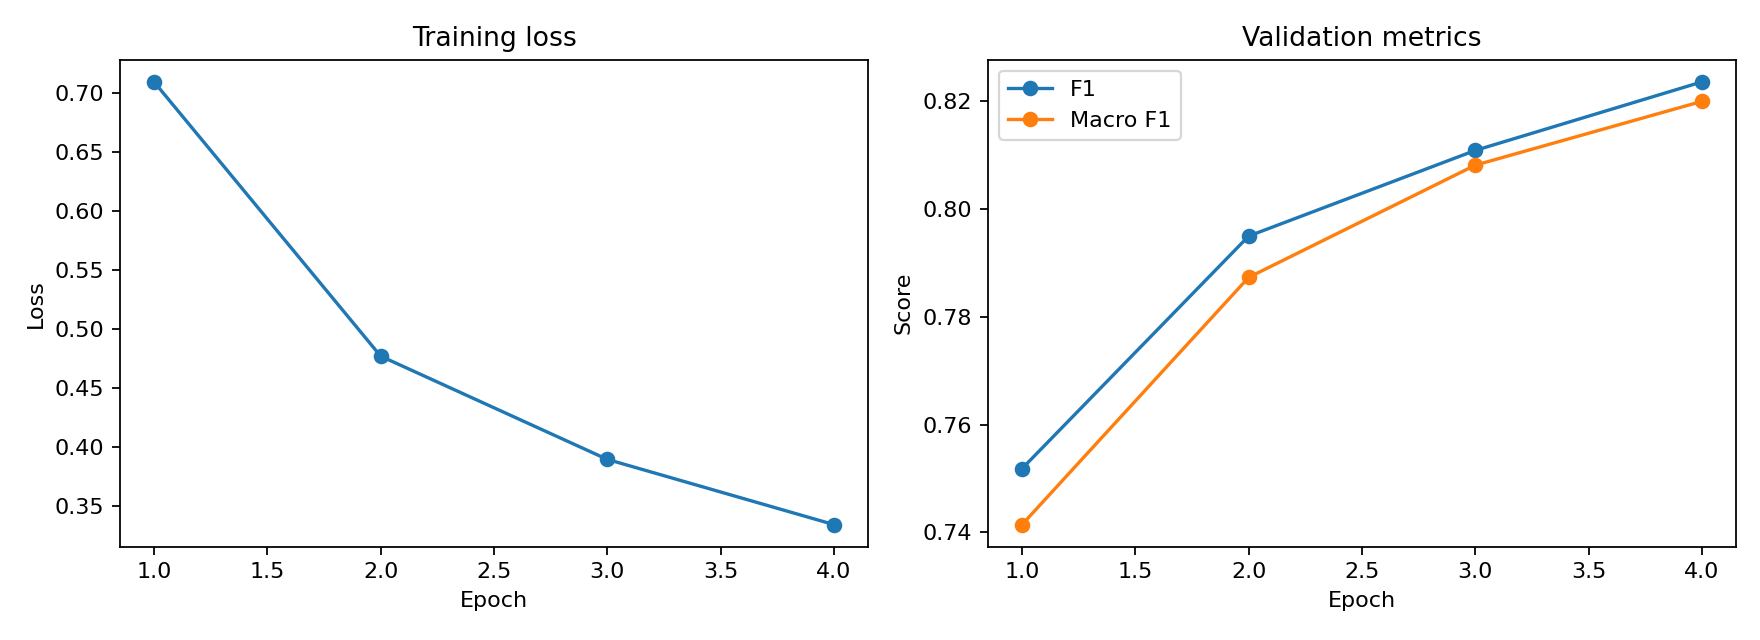
\includegraphics[width=0.95\linewidth]{assets/method_evolution/atcoder_graph_signal_training.png}
\caption{Monotonic loss reduction and simultaneous improvement in F1 and
Macro-F1. The absence of a plateau at epoch four suggests that the run may not
have reached its final performance ceiling.}
\end{figure}

\section{Three-stage AtCoder comparison}

\begin{table}[H]
\centering
\small
\begin{tabular}{lrrrrl}
\toprule
AtCoder version & P & R & F1 & Acc & Attribution status \\
\midrule
Historical Topology only & 0.511 & 0.989 & 0.673 & 0.520 & Nearly all-positive \\
Historical Graph + labels & 0.758 & 0.914 & 0.829 & 0.811 & Direct latent-state bypass \\
Historical Graph + labels + source & 0.813 & 0.929 & 0.867 & 0.858 & Latent and source bypasses \\
First redesign: adjacency-only & 0.500 & 1.000 & 0.667 & 0.500 & Clean spectral path, full collapse \\
Second redesign: graph-signal & 0.795 & 0.872 & 0.832 & 0.824 & Spectral signal, no direct bypass \\
\bottomrule
\end{tabular}
\caption{Historical rows and the two redesigns. Protocol differences limit
direct causal attribution across historical and current rows.}
\end{table}

Relative to adjacency-only, the second redesign improves F1 by 0.165,
Accuracy by 0.324, Macro-F1 by 0.490, and ROC-AUC by 0.395. The positive rate
drops from 100 percent to 54.9 percent. The redesign recovers 82.5 percent of
the F1 gap and 90.4 percent of the Accuracy gap between adjacency-only and the
best historical hybrid configuration. It also exceeds the historical
Graph + labels model without source lexical by 0.003 F1 and 0.013 Accuracy,
while remaining 0.035 F1 below the strongest historical configuration that
used a direct source-lexical residual.

\begin{figure}[H]
\centering
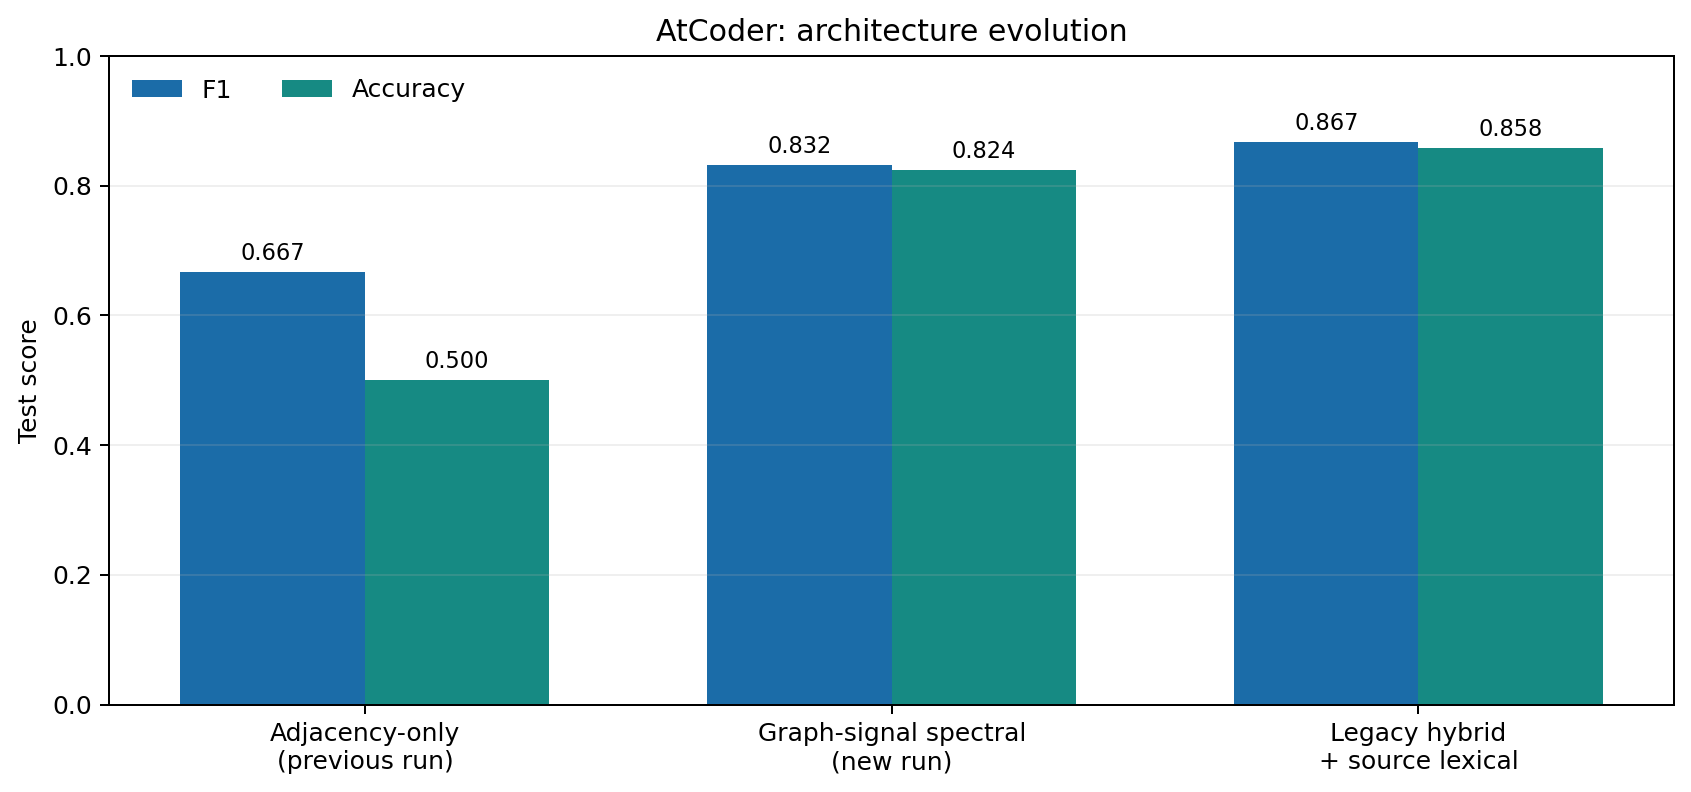
\includegraphics[width=0.91\linewidth]{assets/method_evolution/atcoder_method_comparison.png}
\caption{Recovery of most legacy hybrid performance without restoring a direct
lexical path. The legacy column is a historical reference, not a matched
same-protocol rerun.}
\end{figure}

\begin{keybox}{Current verdict}
The first redesign failed, but the paper's latent graph-representation idea did
not fail. The second redesign shows that semantic attributes can be retained
without an independent feature branch when they are treated as graph signals
and processed by spectral operators. The currently supported claim is that the
new method removes representation collapse and produces a useful attributed
spectral embedding. A claim of universal superiority, or attribution of the
entire gain to one component, still requires matched ablations and multiple
seeds.
\end{keybox}

The computational cost is modest. Parameter count increases from approximately
3,006,221 to 3,013,429, an addition of 7,208 parameters or 0.24 percent.
AtCoder runtime increases from approximately 104.3 minutes in the previous run
to 117.4 minutes, or about 12.5 percent.

\section{Experiments required for scientific attribution}

At minimum, the following arms should use the same split, seed set, training
budget, threshold search, and checkpoint rule.

\begin{enumerate}
\item \textbf{Topology control:} remove canonical and lexical attributes.
\item \textbf{Adjacency-spectrum control:} use canonical and lexical inputs to
construct $A_\Theta$, but expose only adjacency-spectrum statistics.
\item \textbf{Attributed spectral model:} use only
$[d(\lambda),h(\lambda),E(g_b(L)X)]$.
\item \textbf{Hybrid latent control:} add $\mean(Z')$ to the attributed
spectral arm.
\item \textbf{Source lexical control:} add the source-token residual to the
hybrid latent arm.
\item \textbf{Laplacian dependence test:} permute or replace $L$ during
evaluation while preserving $X$.
\item \textbf{Signal dependence test:} exchange $X$ between programs while
preserving $L$.
\item \textbf{Soft-adjacency control:} compare soft weighted adjacency with the
old fixed top-k graph while keeping the readout constant.
\item \textbf{Selection-rule control:} compare positive-F1 checkpoint selection
with ROC-AUC and Macro-F1 selection on identical epoch histories.
\end{enumerate}

If the attributed spectral arm exceeds the adjacency-spectrum control, node
attributes add useful information in the spectral domain. If the hybrid latent
control then improves further, that difference estimates the contribution of
the direct node-state path. The Laplacian and signal dependence tests determine
whether performance truly depends on the interaction between $L$ and $X$.

The next experimental priorities are:
\begin{enumerate}
\item run the graph-signal model on SemanticCloneBench for the configured
30-epoch schedule;
\item rerun AtCoder beyond four epochs because the best checkpoint is the final
reported epoch and validation AUC is still rising;
\item report at least three seeds, preferably five, with mean and standard
deviation;
\item retain Macro-F1, Balanced Accuracy, ROC-AUC, probability standard
deviation, predicted-positive rate, and confusion matrices in every result;
\item compare all key readout arms under one locked protocol before replacing
historical paper tables.
\end{enumerate}

\section{Paper-ready methodology statement}

The revised SPECTRA-Siam encoder represents each program by an attributed
weighted latent graph. Canonical node categories and bounded hashed node-label
features are contextualized over AST and DDG relations and mapped by slot
attention to 32 program-conditioned latent nodes. Their affinities, together
with an assignment-projected structural prior, define a differentiable soft
latent adjacency. The refined latent states are projected to eight graph-signal
channels and filtered by twelve fixed degree-12 Chebyshev approximations of
Gaussian spectral bands on the normalized latent Laplacian. Only the
permutation-invariant log-energy of each filtered channel, concatenated with
32 eigenvalue-density and 24 heat-trace statistics, is projected to the final
code embedding. Pooled latent-node states, input-conditioned band attention,
and source-lexical residuals are excluded from the readout. Consequently, node
attributes can affect prediction only through latent graph induction and their
responses to graph-spectral operators.

\section{Implementation traceability}

\begin{longtable}{p{0.35\linewidth}p{0.57\linewidth}}
\toprule
Method component & Implementation symbol or path \\
\midrule
\endhead
Revised configuration & \code{READOUT\_MODE = "graph\_signal\_spectral"} \\
Node-level lexical input & \code{USE\_NODE\_LEXICAL = True} \\
Source residual removed & \code{USE\_SOURCE\_LEXICAL = False} \\
AST and DDG input & \code{INPUT\_RELATION\_INDICES = [0, 2]} \\
Relational message passing & \code{RelationGraphLayer} \\
Latent-node assignment & \code{SlotAttentionInduction} \\
Soft latent adjacency & \code{CanonicalSpectraEncoder.forward} \\
Spectral filtering and energy & \code{MultiScaleSpectralExtractor} \\
Direct state fusion removed & \code{graph\_signal\_spectral} encoder branch \\
Checkpoint ordering & \code{ROC\_AUC, MacroF1, BalancedAccuracy} \\
Threshold ordering & \code{MacroF1, BalancedAccuracy, F1} \\
SemanticCloneBench notebook & \url{kaggle/semanticclonebench_v3/method/spectra_siam_lex.ipynb} \\
AtCoder notebook & \url{kaggle/atcoder_v3/method/spectra_siam_lex.ipynb} \\
New AtCoder archive & \url{atcoder result.zip} \\
Adjacency-only archive & \url{results.zip} \\
\bottomrule
\end{longtable}

\section{Final assessment}

\begin{itemize}
\item The legacy method allowed canonical and lexical attributes to improve
graph induction, but also exposed a direct latent-state route and, in one
configuration, a source-lexical residual.
\item The adjacency-only redesign removed the attribution ambiguity but also
removed too much semantic information and collapsed on both inspected runs.
\item The graph-signal redesign preserves attributes while constraining their
use to graph-spectral responses.
\item The final representation is spectral, but the correct label is
\emph{attributed graph-spectral}, not \emph{eigenvalue-only}.
\item The AtCoder result demonstrates that the new method removes collapse and
reaches F1=0.832, Accuracy=0.824, Macro-F1=0.823, and ROC-AUC=0.893.
\item Because the best checkpoint is the final epoch, longer training and
multiple seeds remain necessary for a stable final estimate.
\item Matched ablations must separate the contributions of graph-signal energy,
soft adjacency, fixed bands, and checkpoint selection before making a strong
causal claim in the paper.
\end{itemize}

\end{document}
